\chapter{Vehicle routing problem introduction}
\label{chapter:background} 

\begin{figure}[h]
  \begin{center}
    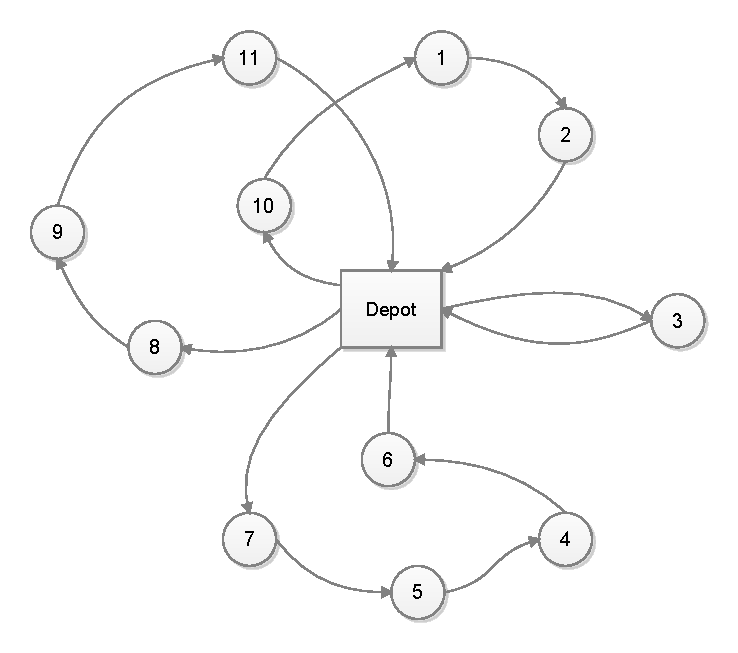
\includegraphics{images/vrpbasic.pdf}
    \caption{An example of a VRP solution}
    \label{fig:simplenetwork}
  \end{center}
\end{figure}

\section{Classical vehicle routing problem}



The basic VRP can be defined with an graph $G = (V, A)$ where $V = \{v_1, v_2, v_3\dots\}$ represents the vertices, ie. the depot and targets for the visitations and $A = \{(v_i, v_j): i \neq j \}$ represents the arcs between the vertices. The vertex $v_0$ typically represents the depot. For every arc, there is a non-negative travel cost $C=(c_{ij})$. In this context, it is used to represent the traveling time between vertices. If the travel cost is symmetric between all pairs of vertices, an undirected graph $G = (V, E)$ can be used instead, where $E=\{(i, j) : i, j \in V, i < j\}$. In all cases, the end result is an all-to-all network. \cite{laporte2007you} 

The main idea in the network is that every node (i.e. vertex) has a connecting edge to every other node. Even if in real life there would be overlapping in the routes as one road probably leads to more than just one node, for the sake of the problem the edges are considered unique, as can be seen in Figure~\ref{fig:reallifenetwork}. In other words, even though the road map of a country does not consist of an all-to-all type network topology, the mathematical model used for this problem uses one. 

\begin{figure}[h]
  \begin{center}
    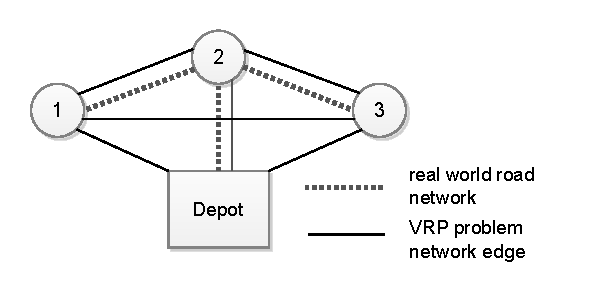
\includegraphics{images/simplenetwork.pdf}
    \caption{Real life network and the mathematical network}
    \label{fig:reallifenetwork}
  \end{center}
\end{figure}

The first vertex in $V$ represents the depot, where all the vehicles start from and where they must end their trips. $m$ identical vehicles have a capacity denoted by $Q$ which symbolises the resources available for each trip. In the classic VRP, $m$ is logically equivalent to the number of trips needed to visit every customer. With time windows this no longer holds true. Every customer vertex $i \in V\setminus\{v_0\}$ has a demand $q_i \leq Q$ associated with it. This symbolises the various resources, including time, required at the target. \cite{laporte2007you}

Vehicle routing problem is NP-hard as it is a superset of the traveling salesman problem. In traveling salesman problem, the number of vehicles is $m = 1$, there is no upper limit on the costs of a route and the capacity of the vehicle is greater than the combined requirement of all the nodes in the network ($Q = \infty$). \cite{laporte2007you} The classic VRP is sometimes called the capacitated vehicle routing problem (CVRP). \cite{hassanzadeh2009location}

Let $x_{ij}$ denote the number of trips made over the edge $[i, j]$ in a solution. The total cost that should be minimised is then:

\begin{equation}
\label{eq:baseformula1}
\displaystyle \sum_{[i,j] \in E} c_{ij}x_{ij}.
\end{equation}

\noindent
The following conditions must hold true:

\begin{equation}
\label{eq:baseformula2}
\displaystyle \sum_{j \in V \setminus\{0\}} x_{0j} = 2m,
\end{equation}

\noindent
meaning that given $m$ routes, the edges between the depot and other vertices are used exactly $2m$ times, as seen in Figure~\ref{fig:basecond1}. \cite{laporte2007you}
\begin{figure}[h]
  \begin{center}
    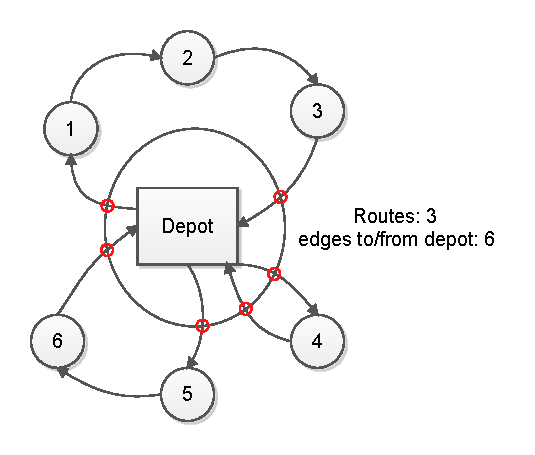
\includegraphics{images/basecond1.pdf}
    \caption{Routes to and from the depot}
    \label{fig:basecond1}
  \end{center}
\end{figure}

\begin{equation}
\begin{aligned}
\label{eq:baseformula3}
\displaystyle\sum_{i < k} x_{ik} + \displaystyle\sum_{j > k} x_{kj} = 2 && (k \in V \setminus\{0\}),
\end{aligned}
\end{equation}

\noindent
meaning that every vertex that is not the depot has two connecting edges that are used in the solution. In other words, every non-depot vertex is visited exactly once. \cite{laporte2007you}

\medskip
\noindent
If $b(S)$ represents the minimum number of vehicles required to satisfy the needs of the customers of $S$, the constraint

\begin{equation}
\begin{aligned}
\label{eq:baseformula4}
\displaystyle\sum_{\substack{i \in S, j \notin S \\ 
\text{ or } i \notin S, j \in S}} x_{ij} \geq 2b(S) && (S \subset V \setminus\{0\}).
\end{aligned}
\end{equation}

\noindent
means the number of edges travelled between the vertices in the network contained in S and the vertices of the rest of the network has to be at least 2 times the minimum number of vehicles required to satisfy the needs of the customers of $S$. \cite{laporte2007you}



\begin{equation}
\begin{aligned}
\label{eq:baseformula5}
x_{i,j} = 0 \text{ or } 1 && (i, j \in V\setminus\{0\})
\end{aligned}
\end{equation}

\noindent
and

\begin{equation}
\begin{aligned}
\label{eq:baseformula6}
x_{0,j} = 0, 1 \text{ or } 2 && (j \in V\setminus\{0\})
\end{aligned}
\end{equation}

\noindent
mean that every edge whose other end is the depot is travelled at most two times, while the rest of the edges are traveled once at most. \cite{laporte2007you}







\section{Variations of the vehicle routing problem}

The real life needs of route planning are rarely satisfied with the basic vehicle routing problem. There are typically additional constraints and an increased complexity that require expanding the problem statement. The vehicles used are probably not identical in terms of capacity and cost. The number of depots might also be greater than 1 and each target has to be allocated to one of them. \cite{salhi2014multi} In addition, there might be specific time windows during which the targets have to be visited \cite{ghoseiri2010multi}. 

All of these additional features can be combined into a multitude of variations of the VRP. As all the variations add to the complexity of the VRP, they too are NP-hard. The variations listed here represent the most common types of VRP, but in addition, there are more specific types still available, such as one where only certain types of vehicles may visit certain targets. \cite{montoya2015literature} 


\subsection{Multi-depot Vehicle routing problem}

Multi-depot Vehicle routing problem (MDVRP) is a variation of VRP where there are additional depots which can be utilised as the start and end points of routes as can be seen in Figure~\ref{fig:multidepot}. A vehicle must start and end the route at the same depot. While at first it might seem that MDVRP can be just split into multiple single depot VRPs by assigning each target to the nearest depot, this leads to suboptimal solutions. \cite{salhi2014multi}

\begin{figure}[h]
  \begin{center}
    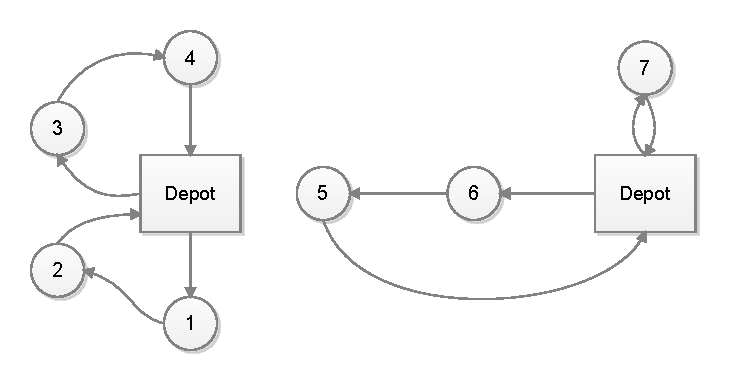
\includegraphics{images/multidepot.pdf}
    \caption{A VRP with two depots}
    \label{fig:multidepot}
  \end{center}
\end{figure}

\subsection{Heterogenous fleet vehicle routing problem}

In real world scenarios, it is uncommon that all the vehicles in a fleet are identical. A typical variation of the VRP called heterogenous fleet vehicle routing problem (HVRP) one where the vehicles are not assumed to be identical. There is a fixed cost associated with each vehicle type and a variable cost per distance unit. Vehicle types also have unique capacities which play an important role in route generation. \cite{gendreau1999tabu}


\subsection{Vehicle routing problem with time windows}

Time windows and other scheduling constraints are common in real world and thus including them in VRP is crucial in order to get results that are applicable in common business cases. These can include postal, food or cargo delivery and service visits where it is common that the customer wants the delivery to occur during a specific time. \cite{cordeau2000vrp}

To define vehicle routing problem with time windows (VRPTW), let $s_i$ denote the time that a vehicle has to spend at a target $i$ and $b_i$ denote the time at which the delivery of the service or goods begins. The earliest time the target accepts the start of the delivery is $e_i$ and the latest is $l_i$. If a vehicle arrives too early at $j$, it will have to wait so that the earliest time it can deliver the goods or services is $b_i = \max\{e_j, b_i + s_i + t_{ij}\}$. Here $t_{ij}$ represents the time required to travel between $i$ and $j$. \cite{solomon1987algorithms}


\subsection{Vehicle routing problem with pickup and delivery}

Vehicle routing problem with pickup and delivery (VRPPD) defines a VRP where a set of transportation requests must be satisfied. The requests all have a pickup point and a delivery point where the goods or passenger has to be brought. In case of passengers, a common application in real life can be found in taxi service. A courier service would be an example of a scenario where goods need to be transported from one point to another. Due to the nature of the applications for VRPPD, it is usually combined with VRPTW. The standard VRP is a VRPPD where the pickup point is always the depot and the delivery points are spread out elsewhere or vice versa. \cite{desaulniers2000vrp}


\subsection{Periodic vehicle routing problem}

While the classic VRP assumes a single time period, a single day for example, during which a deliveries have to be made, periodic vehicle routing problem (PVRP) defines a case with repeating time windows. Customers may need to be visited once or multiple times, and they may require the visit to occur on a specific weekday. \cite{blakeley2003optimizing} Common applications for the PVRP include waste collection, vending machine replenishment and cleaning service. PVRP is commonly combined with VRPTW as it is likely that in addition to wanting the visit to take place on a specific day, the customers also have requirements regarding the time of the visit. \cite{yu2011ant}


\subsection{Location routing problem}

In location routing problem (LRP), the location of the depots has to be determined before creating the routes. The factors that have to be taken into account are the one time and running costs of the depots and the traveling costs that are based on the locations of the depots. The main objective is to position the depots as close to the customers as possible. In practice, the maximum size of the depot is also limited. A large depot in a city centrum might incur too large costs in order to be feasible. Once the locations of the depots has been decided, the problem turns into a multi-depot vehicle routing problem, though naturally the positions can be altered at any point during the solving. \cite{tuzun1999two}


\subsection{Green vehicle routing problem}

Due to the apparent need to cut down $CO^2$ emissions and the fact that the vast majority of vehicles, especially heavy transport, run on fossil fuels, there is an increasing motivation to pay more attention to the environmental aspects of transportation. Green vehicle routing problem (GVRP, also known as emissions vehicle routing problem) aims to minimise emissions and helps routing for vehicles that may require special fueling stations. \cite{erdougan2012green}



\section{VRP solutions}

In this section I present some common algorithms to produce solutions to various VRPs. Because there are so many different types of VRP and each having its own set of solving methods, only the most common ones are listed here. In chapter~\ref{chapter:implementation} I will more closely analyse which additional VRP features are required in the business case of this thesis. Then I will analyse which of these solutions methods will be most suitable to produce usable solutions.

There are three main categories of VRP solving algorithms. The first category consists of algorithms that produce exact solutions. Due to the complexity of VRP, exact algorithms can only handle networks with up to about 100 nodes. This has resulted in the bulk of the research focusing on the two main types of heuristics: Classical heuristics and metaheuristics. \cite{laporte2007you}  

Classical heuristics produce good results in reasonable computing time and cover the bulk of most modern heuristics in use. They are also easily suited for real world constraints and requirements. In metaheuristics, the most promising solution space is further explored. They employ advanced neighbourhood search patterns, memory structures and commonly use recombinations of solutions to find better ones. The downside is increased complexity and computational requirements, but they typically produce higher quality solutions. \cite{laporte2000classical}

For notation, we will use (0, $i$, $j$, $k$, 0) to denote a route that starts at depot 0 and goes to targets $i$, $j$ and $k$ before returning to the depot. In case of multiple depots, they will be denoted with other indexes, e.g. (1, $l$, $m$, 1).



\subsection{Savings algorithm}

The savings algorithm is one of the most basic algorithms for VRP. It assumes that the number of vehicles is a decision variable. Figure~\ref{fig:savings1} shows an example of how the savings algorithm progresses.

\begin{figure}[h]
  \begin{center}
    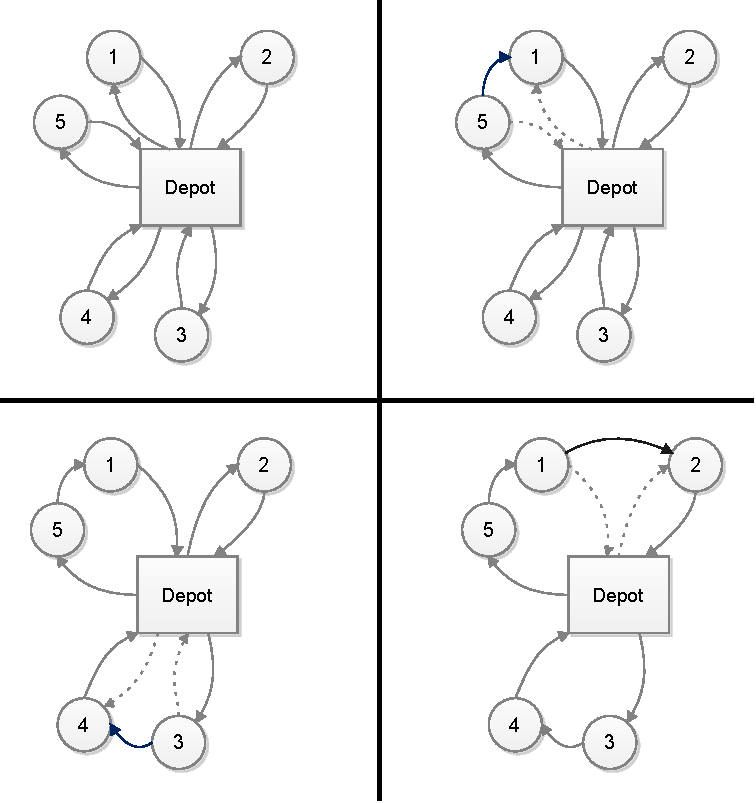
\includegraphics{images/Savings1.pdf}
    \caption{An example of savings algorithm progression where car capacity is 3 and demand per node is 1}
    \label{fig:savings1}
  \end{center}
\end{figure}

\bigskip
\noindent
Create one vehicle route per node so that the route just goes to the target and comes back to the depot. This will result in $n$ vehicle routes (0, $i$, 0) for $i = 1, \ldots, n$. \cite{reimann2004d}

\medskip
\noindent
\textbf{Step 1:} Calculate \textit{savings}: $s_{ij} = c_{i0} + c_{0j} - c_{ij} \text{ for } i, j = 1, \ldots, n \text{ and } i \neq j$. Sort the savings in descending order. \cite{reimann2004d} At the top of the savings list are then pairs of targets who are farthest away from the depot and closest to each other. Essentially this gives us the clue that they should probably be merged into the same route. There are two common ways to use the savings list.


\medskip
\noindent
\textbf{Step 2 (best savings first):} Starting from the top of the savings list, see if the routes can be merged so that the saving $s_{ij}$ causes the removal of $(0, j)$ and $(i, 0)$ and the addition of $(i, j)$. \cite{reimann2004d} This means that no routes will be cut in half during the algorithm, but that routes are merged from end to end, excluding the depot.

\medskip
\noindent
\textbf{Step 2 (route first):} For each route $(0, i, \ldots, j, 0)$, find the first saving $s_{ki}$ or $s_{jl}$ that allows merging of another route that either ends with $(k, 0)$ or starts with $(0, l)$. Merge these two routes and continue the operation until no more feasible merges exist. Then move on to the next route and start all over again. \cite{laporte2000classical}

 



\subsection{Sweep algorithm}			

Popularised by Gillet and Miller in 1974, the sweep algorithm is usable on data sets where the coordinates of the targets are known. It is based on calculating the polar coordinates between the depot and the targets so that one arbitarily chosen target represents the zero angle. The targets are then sorted according to the polar angle. The sorted targets are added in order to the new route until the cost or capacity limit of a single route has been reached and no more new targets can be inserted. Then a new route is created and the algorithm is repeated until all targets have been assigned to a route. \cite{gillett1974heuristic}

The found routes are then optimised with any traveling salesman solver. Since the routes are supposedly relatively small at this point, solving the individual TSPs should be a lightweight operation. Once each route has been initially created and optimised, the algorithm then tries to swap neighbour routes' targets according to their distance from the depot and the angle to the next route. If the swap improves the solution, the target is moved to the other route. After no more improvements can be found through swapping, the algorithm finishes. \cite{gillett1974heuristic} Figure~\ref{fig:sweep1} shows an example of how the sweep algorithm works in practice. 

The downside to this heuristic is that it doesn't take the road network into account during the sweep. It assumes that the geometrical distance is the most important piece of criteria. To counter this, it is typical to run the algorithm so that all targets get picked to be as the beginning point of the sweep. \cite{reimann2004d} 


\begin{figure}[h]
  \begin{center}
    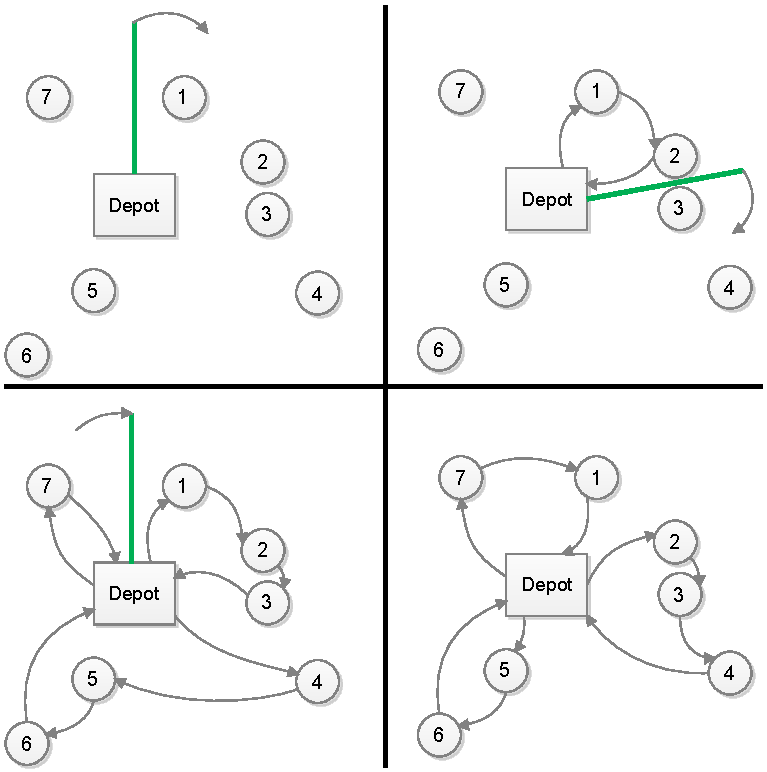
\includegraphics{images/Sweep1.pdf}
    \caption{An example of sweep algorithm progression where car capacity is 3 and demand per node is 1. In the final iteration some routes swap nodes to produce more optimal solution.}
    \label{fig:sweep1}
  \end{center}
\end{figure}

\subsection{Petal algorithm}

The petal algorithm resembles the sweep algorithm, as all the targets are first sorted according to their polar angle from the depot and an arbitarily chosen point. A set $S$ of possible routes called petals is then generated and optimised using TSP as above. The problem is then formulated as follows:


\bigskip
\noindent
Minimise

\begin{equation}
\label{eq:petal1}
\displaystyle\sum_{\substack{k \in S}} d_kx_k
\end{equation}


\noindent
where $S$ is the set of all routes in the set, $x_k = 1$ if and only if route k is part of the solution and $d_k$ represents the cost of the whole route $k$. Apply the following conditions:

\begin{equation}
\begin{aligned}
\label{eq:petal2}
\displaystyle\sum_{\substack{k \in S}} a_{ik}x_k = 1 && i = 1, \ldots, n
\end{aligned}
\end{equation}

\noindent
and

\begin{equation}
\begin{aligned}
\label{eq:petal3}
x_{k} = 0 \text{ or } 1 && k \in S
\end{aligned}
\end{equation}

where $a_{ik}$ is 1 only if the vertex $i$ is in the route $k$. \cite{laporte2000classical} The conditions state that every vertex belongs to exactly one route. The Sweep and petal algorithms are classic examples of ``cluster-fist route-second'' types of algorithms, where first the targets are grouped and then for those groups, the optimal routes are discovered. 

\subsection{2-petal algorithm}

\subsection{Tabu search}

\subsection{Greedy Randomized Adaptive Search Procedure (GRASP)}

\subsection {Ruin and Recreate}

\label{subsection:ruinandrecreate} 

Developed by Schrimpf et al., the ruin and recreate algorithm is based on the concept of having a solution of varying quality as the base, after which all trips to a set of nodes are removed (``ruined''). The set can be picked randomly, from a radial area, or by some other rule. The intermediate result is the same solution as in the beginning, with some nodes not being serviced. The routes are then re-created so that every ruined node gets inserted into a route where it creates the least amount of additional time requirement so that no constraints (capacity, time, etc.) are broken. If it is impossible to insert a ruined node to a route without breaking constraints, a new route will be created. Once all the ruined nodes have been readded to routes, the algorithm can be repeated. \cite{schrimpf2000record} 

Shrimpf et al. state that there are probably better and more elaborate algorithms for the recreation procedure, but that even with their simple scheme, very good results can be achieved. Likewise, there are numerous strategies to choose from for the ruin part of the algorithm. Also, choosing which solution to continue from after iterations affects results. One way is to always use the best results gotten so far, but it may also pay off to try to continue from a slightly worse solution. A big benefit of the algorithm is that it allows easy applying of custom constraints. \cite{schrimpf2000record} 

This algorithm is used in the library I picked to use for the VRP program. In addition it employs features presented by Pisinger and Ropke\cite{pisinger2007general}.

TODO: add graph demonstration, expand on the various strategies in the phases of the algorithm.

\subsection{Genetic algorithm}

\subsection{Ant colony}

\subsection{Bee colony}